\chapter{Shape-from-Shading}
\label{ch:sfs}

ASP provides a tool, named \texttt{sfs}, that can improve the level of
detail of DEMs created by ASP or any other source using
\textit{shape-from-shading} (SfS). The tool takes as input one or more
camera images, a DEM at roughly the same resolution as the images, and
returns a refined DEM.

\texttt{sfs} works only with ISIS cub images. It has been tested
thoroughly with Lunar LRO NAC datasets, and some experiments were done
with Mars HiRISE images and with pictures from Charon, Pluto's moon. As
seen later in the text, it returns reasonable results on the Moon as far
as $85^\circ$ and even $89.6^\circ$ South.

Currently, \texttt{sfs} is computationally expensive, and is practical
only for DEMs whose width and height are several thousand pixels. It can be 
sensitive to errors in the position and orientation of the cameras, the
accuracy of the initial DEM, and to the value of the two weights it uses.
Yet, with some effort, it can work quite well. 

A tool named \texttt{parallel\_sfs} is provided (section \ref{psfs}) 
that parallelizes \texttt{sfs} using multiple processes (optionally on
multiple machines) by splitting the input DEM into tiles with padding,
running \texttt{sfs} on each tile, and then blending the results. 

The \texttt{sfs} program can model position-dependent albedo, different
exposure values for each camera, shadows in the input images, and regions
in the DEM occluded from the Sun. It can refine the positions and orientations
of the cameras.

The tool works by minimizing the cost function
\begin{equation}\label{cost}
  % \begin{multline}\label{cost}
  \int\!\! \int \! \sum_k \left[ I_k(\phi)(x, y) - T_k A(x, y)
    R_k(\phi)(x, y) \right]^2\,  
  % R_k(\phi)(x, y) \right]^2\,  \\
  + \mu \left\|\nabla^2 \phi(x, y) \right\|^2  
  + \lambda  \left[ \phi(x, y) - \phi_0(x, y) \right]^2
  \, dx\, dy.
\end{equation}
% \end{multline}

Here, $I_k(\phi)(x, y)$ is the $k$-th camera image interpolated at
pixels obtained by projecting into the camera 3D points from the terrain
$\phi(x, y)$, $T_k$ is the $k$-th image exposure, $A(x, y)$ is the
per-pixel albedo, $R_k(\phi)(x, y)$ is the reflectance computed from the
terrain for $k$-th image, $\left\|\nabla^2 \phi(x, y) \right\|^2 $ is the sum
of squares of all second-order partial derivatives of $\phi$, $\mu > 0$
is a smoothing term, and $\lambda > 0$ determines how close we should
stay to the input terrain $\phi_0$ (smaller $\mu$ will show more detail
but may introduce some artifacts, and smaller $\lambda$ may allow for
more flexibility in optimization but the terrain may move too far from the input). 

We use either the regular Lambertian reflectance model,
or the Lunar-Lambertian model \cite{mcewen1991photometric}, more specifically as given in
\cite{lohse2006derivation} (equations (3) and (4)).
Also supported is the Hapke model, 
\cite{johnson2006spectrophotometric}, \cite{fernando2013surface},
\cite{hapke2008bidirectional}, \cite{hapke1993opposition}.
Custom values for the coefficients of these models can be passed to the program.

\section{How to get good test imagery}

We obtain the images from
\url{http://wms.lroc.asu.edu/lroc/search} (we search for EDR images of
type NACL and NACR). 

A faster (but not as complete) interface is provided by
\url{http://ode.rsl.wustl.edu/moon/indexproductsearch.aspx}. The related
site
\url{http://ode.rsl.wustl.edu/moon/indextools.aspx?displaypage=lolardr}
can provide LOLA datasets which can be used as (sparse) ground truth.

We advise the following strategy for picking images. First choose a small
longitude-latitude window in which to perform a search for imagery. Pick
two images that are very close in time and with a big amount of overlap
(ideally they would have consecutive orbit numbers).
Those can be passed to ASP's \texttt{stereo} tool to create an initial DEM. Then, search for 
other images close to the center of the maximum overlap of the first
two images. Pick one or more of those, ideally with different illumination
conditions than the first two. Those (together with one of the first two images) can be used for SfS.

To locate the area of spatial overlap, the images can be map-projected (either
with \texttt{cam2map} with a coarse resolution) or with
\texttt{mapproject}, using for example the LOLA DEM as the terrain to project onto, 
or the DEM obtained from running \texttt{stereo} on those images. Then the images can be overlayed
in \texttt{stereo\_gui}. A good sanity check is to examine the shadows in
various images. If they point in different directions in the images and perhaps
also have different lengths, that means that illumination conditions are
different enough, which will help constrain the \texttt{sfs} problem better.

\section{Running sfs at 1 meter/pixel using a single image}

In both this and the next sections we will work with LRO NAC images taken
close to the Lunar South Pole, at a latitude of $85^\circ$ South (the tool was
tested on equatorial regions as well). We will use four images,
M139939938LE, M139946735RE, M173004270LE, and M122270273LE.

We first retrieve the data sets.
\begin{verbatim}
  wget http://lroc.sese.asu.edu/data/LRO-L-LROC-2-EDR-V1.0/\
LROLRC_0005/DATA/SCI/2010267/NAC/M139939938LE.IMG
  wget http://lroc.sese.asu.edu/data/LRO-L-LROC-2-EDR-V1.0/\
LROLRC_0005/DATA/SCI/2010267/NAC/M139946735RE.IMG
  wget http://lroc.sese.asu.edu/data/LRO-L-LROC-2-EDR-V1.0/\
LROLRC_0009/DATA/SCI/2011284/NAC/M173004270LE.IMG
  wget http://lroc.sese.asu.edu/data/LRO-L-LROC-2-EDR-V1.0/\
LROLRC_0002/DATA/MAP/2010062/NAC/M122270273LE.IMG
\end{verbatim}

Then we convert them to ISIS cubes, initialize the SPICE kernels, and
perform radiometric calibration and echo correction. Here are the steps, 
illustrated on the first image:
\begin{verbatim}  
  lronac2isis from = M139939938LE.IMG     to = M139939938LE.cub
  spiceinit   from = M139939938LE.cub
  lronaccal   from = M139939938LE.cub     to = M139939938LE.cal.cub
  lronacecho  from = M139939938LE.cal.cub to = M139939938LE.cal.echo.cub
\end{verbatim}
We rename, for simplicity, the obtained four processed datasets to
A.cub, B.cub, C.cub, and D.cub.

The first step is to run stereo to create an initial guess DEM. We
picked for this the first two of these images. These form a stereo pair,
that is, they have a reasonable baseline and sufficiently close times of
acquisition (hence very similar illuminations). These conditions are
necessary to obtain a good stereo result.
\begin{verbatim}
parallel_stereo --job-size-w 1024 --job-size-h 1024 A.cub B.cub    \
                --left-image-crop-win 0 7998 2728 2696             \
                --right-image-crop-win 0 9377 2733 2505            \
                --threads 16 --corr-seed-mode 1  --subpixel-mode 3 \
                run_full1/run
\end{verbatim}
Next we create a DEM at 1 meter/pixel, which is about the resolution
of the input images. We use the stereographic projection since this
dataset is very close to the South Pole. Then we crop it to the region
we'd like to do SfS on.
\begin{verbatim}
  point2dem -r moon --stereographic --proj-lon 0 \
    --proj-lat -90 run_full1/run-PC.tif
  gdal_translate -projwin -15471.9 150986 -14986.7 150549  \
    run_full1/run-DEM.tif run_full1/run-crop-DEM.tif
\end{verbatim}
This creates a DEM of size $456 \times 410$ pixels.

Then we run \texttt{sfs}:
\begin{verbatim}
  sfs -i run_full1/run-crop-DEM.tif A.cub -o sfs_ref1/run           \
     --reflectance-type 1                                           \
    --smoothness-weight 0.08 --initial-dem-constraint-weight 0.0001 \
    --max-iterations 10 --use-approx-camera-models                  \
    --use-rpc-approximation --crop-input-images  
\end{verbatim}

The smoothness weight is a parameter that needs tuning. If it is too
small, SfS will return noisy results, if it is too large, too much
detail will be blurred. Here we used the Lunar Lambertian model. The
meaning of the other \texttt{sfs} options can be looked up in section
\ref{sfs}.

We show the results of running this program in figure
\ref{fig:sfs1}. The left-most figure is the hill-shaded original DEM,
which was obtained by running:
\begin{verbatim}
  hillshade --azimuth 300 --elevation 20 run_full1/run-crop-DEM.tif \
    -o run_full1/run-crop-hill.tif 
\end{verbatim}
The second image is the hill-shaded DEM obtained after running
\texttt{sfs} for 10 iterations.

The third image is, for comparison, the map-projection of A.cub onto the
original DEM, obtained via the command:
\begin{verbatim}
  mapproject --tr 1 run_full1/run-crop-DEM.tif A.cub A_map.tif --tile-size 128
\end{verbatim}
The forth image is the colored absolute difference between the original
DEM and the SfS output, obtained by running:
\begin{verbatim}
  geodiff --absolute sfs_ref1/run-DEM-final.tif run_full1/run-crop-DEM.tif
  colormap --min 0 --max 2 --colormap-style binary-red-blue \
    run-DEM-final__run-crop-DEM-diff.tif
\end{verbatim}
\begin{figure}[h!]
  \begin{center}
    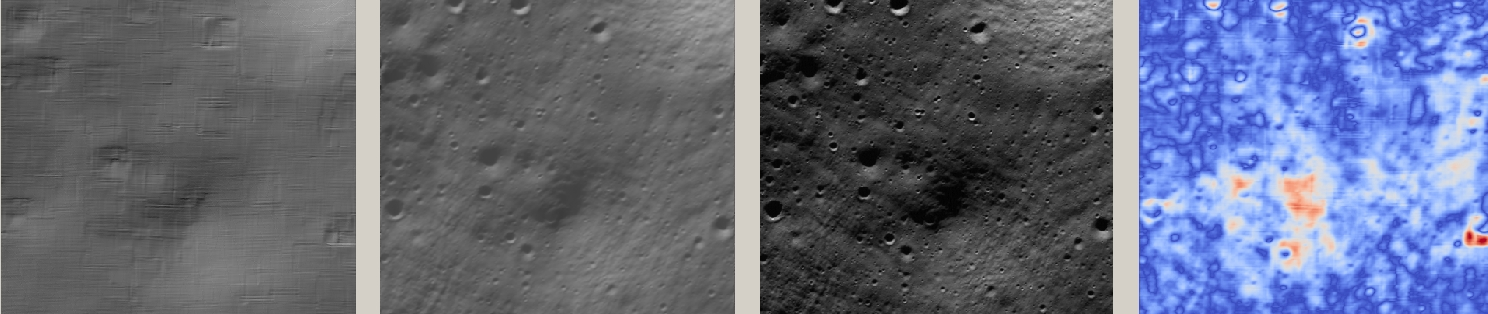
\includegraphics[width=7in]{images/sfs1.jpg}
    \caption[sfs]{An illustration of \texttt{sfs}. The images are, from
      left to right, the original hill-shaded DEM, the hill-shaded DEM obtained
      from \texttt{sfs}, the image A.cub map-projected onto the original DEM,
      and the absolute difference of the original and final DEM, where the brightest
      shade of red corresponds to a 2 meter height difference.}
    \label{fig:sfs1}
  \end{center}
\end{figure}

It can be seen that the optimized DEM provides a wealth of detail and
looks quite similar to the input image. It also did not diverge
significantly from the input DEM. We will see in the next section that
SfS is in fact able to make the refined DEM more accurate than the
initial guess (as compared to some known ground truth), though that is
not guaranteed, and most likely did not happen here where just one image
was used.

\section{SfS with multiple images in the presence of shadows}

In this section we will run \texttt{sfs} with multiple images. We would
like to be able to see if SfS improves the accuracy of the DEM rather
than just adding detail to it. We evaluate this using the following
(admittedly imperfect) approach. We resample the original images by a
factor of 10, run stereo with them, followed by SfS using the stereo
result as an initial guess and with the resampled images. As ground
truth, we create a DEM from the original images at 1 meter/pixel, which
we bring closer to the initial guess for SfS using
\texttt{pc\_align}. We would like to know if running SfS brings us even
closer to this ``ground truth'' DEM.

The most significant challenge in running SfS with multiple images is
that shape-from-shading is highly sensitive to errors in camera position
and orientation. The \texttt{sfs} tool can improve these by floating
them during optimization and by using a coarse-to-fine scheme, where
the problem is first solved using subsampled images and terrain then
it is successively refined.

If possible, it may still be desirable to bundle-adjust the cameras first
(section \ref{bundleadjust}). It is important to note that bundle adjustment may
fail if the images have sufficiently different illumination, as it will
not be able to find matches among images. A solution to this is discussed
in section \ref{sfs-lola}.

To make bundle adjustment and stereo faster, we first crop the images,
such as shown below (the crop parameters can be determined via
\texttt{stereo\_gui}).
\begin{verbatim}
  crop from = A.cub to = A_crop.cub sample = 1 line = 6644 nsamples = 2192 nlines = 4982
  crop from = B.cub to = B_crop.cub sample = 1 line = 7013 nsamples = 2531 nlines = 7337
  crop from = C.cub to = C_crop.cub sample = 1 line = 1 nsamples = 2531 nlines = 8305
  crop from = D.cub to = D_crop.cub sample = 1 line = 1 nsamples = 2531 nlines = 2740
\end{verbatim}
Then we bundle-adjust and run stereo
\begin{verbatim}
  bundle_adjust A_crop.cub B_crop.cub C_crop.cub D_crop.cub    \
    --min-matches 1 -o run_ba/run
  stereo A_crop.cub B_crop.cub run_full2/run --subpixel-mode 3 \
    --bundle-adjust-prefix run_ba/run
\end{verbatim}

This will result in a point cloud, \verb#run_full2/run-PC.tif#, which will
lead us to the ``ground truth'' DEM. As mentioned
before, we'll in fact run SfS with images subsampled by a factor of
10. Subsampling is done by running the ISIS \texttt{reduce} command
\begin{verbatim}
  for f in A B C D; do 
    reduce from = ${f}_crop.cub to = ${f}_crop_sub10.cub sscale = 10 lscale = 10
  done
\end{verbatim}

We run bundle adjustment and stereo with the subsampled images using
commands analogous to the above:
\begin{verbatim}
  bundle_adjust A_crop_sub10.cub B_crop_sub10.cub C_crop_sub10.cub D_crop_sub10.cub \
    --min-matches 1 -o run_ba_sub10/run --ip-per-tile 100000
 stereo A_crop_sub10.cub B_crop_sub10.cub run_sub10/run --subpixel-mode 3           \
   --bundle-adjust-prefix run_ba_sub10/run
\end{verbatim}
We'll obtain a point cloud named \verb#run_sub10/run-PC.tif#.

We'll bring the ``ground truth'' point cloud closer to the initial guess
for SfS using \texttt{pc\_align}:
\begin{verbatim}
  pc_align --max-displacement 200 run_full2/run-PC.tif run_sub10/run-PC.tif \
    -o run_full2/run --save-inv-transformed-reference-points
\end{verbatim}
This step is extremely important. Since we ran two bundle adjustment
steps, and both were without ground control points, the resulting clouds
may differ by a large translation, which we correct here. Hence we would like to 
make the ``ground truth'' terrain aligned with the datasets on which we 
will perform SfS. 

Next we create the ``ground truth'' DEM from the aligned high-resolution
point cloud, and crop it to a desired region:
\begin{verbatim}
  point2dem -r moon --tr 10 --stereographic --proj-lon 0 --proj-lat -90 \
    run_full2/run-trans_reference.tif
  gdal_translate -projwin -15540.7 151403 -14554.5 150473               \
    run_full2/run-trans_reference-DEM.tif run_full2/run-crop-DEM.tif
\end{verbatim}
We repeat the same steps for the initial guess for SfS:
\begin{verbatim}
  point2dem -r moon --tr 10 --stereographic --proj-lon 0 --proj-lat -90 \
    run_sub10/run-PC.tif
  gdal_translate -projwin -15540.7 151403 -14554.5 150473               \
    run_sub10/run-DEM.tif run_sub10/run-crop-DEM.tif
\end{verbatim}
After this, we run \texttt{sfs} itself. Since our dataset has many shadows, we found
that specifying the shadow thresholds for the tool improves the
results. The thresholds can be determined using \texttt{stereo\_gui}.
This can be done by turning on shadow-threshold mode from the GUI menu, 
and then clicking on a few points in the shadows.  Then the thresholded images
can be visualized/updated from the menu as well, and this process can be iterated.
\begin{verbatim}
  sfs -i run_sub10/run-crop-DEM.tif A_crop_sub10.cub C_crop_sub10.cub \
    D_crop_sub10.cub -o sfs_sub10_ref1/run --threads 4                \
    --smoothness-weight 0.12 --initial-dem-constraint-weight 0.0001   \
    --reflectance-type 1 --float-exposure                             \
    --float-cameras --use-approx-camera-models                        \
    --max-iterations 10 --use-approx-camera-models                    \
    --use-rpc-approximation --crop-input-images                       \
    --bundle-adjust-prefix run_ba_sub10/run                           \
    --shadow-thresholds "0.00162484 0.0012166 0.000781663"
\end{verbatim}
We compare the initial guess to \texttt{sfs} to the ``ground truth'' DEM
obtained earlier and the same for the final refined DEM using
\texttt{geodiff} as in the previous section. Before SfS:

\begin{verbatim}
  geodiff --absolute run_full2/run-crop-DEM.tif run_sub10/run-crop-DEM.tif
  gdalinfo -stats run-crop-DEM__run-crop-DEM-diff.tif | grep Mean=  
\end{verbatim}
and after SfS:
\begin{verbatim}
  geodiff --absolute run_full2/run-crop-DEM.tif sfs_sub10_ref1/run-DEM-final.tif
  gdalinfo -stats run-crop-DEM__run-DEM-final-diff.tif | grep Mean=
\end{verbatim}

The mean error goes from 2.64~m to 1.29~m, while the standard deviation
decreases from 2.50~m to 1.29~m. Visually the refined DEM looks more detailed
as well as seen in figure \ref{fig:sfs2}. The same experiment can be
repeated with the Lambertian reflectance model (reflectance-type 0), and
then it is seen that it performs a little worse. 

We also show in this figure the first of the images used for SfS,
\verb#A_crop_sub10.cub#, map-projected upon the optimized DEM. Note that
we use the previously computed bundle-adjusted cameras when
map-projecting, otherwise the image will show as shifted from its true
location:
\begin{verbatim}
  mapproject sfs_sub10_ref1/run-DEM-final.tif A_crop_sub10.cub A_crop_sub10_map.tif \
    --bundle-adjust-prefix run_ba_sub10/run
\end{verbatim}
\begin{figure}[h!]
  \begin{center}
    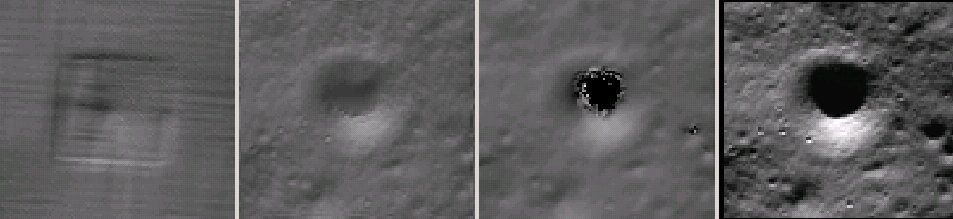
\includegraphics[width=7in]{images/sfs2.jpg}
    \caption[sfs]{An illustration of \texttt{sfs}. The images are, from
      left to right, the hill-shaded initial guess DEM for SfS, the hill-shaded DEM obtained
      from \texttt{sfs}, the ``ground truth'' DEM, and the first of the
      images used in SfS map-projected onto the optimized DEM.}
    \label{fig:sfs2}
  \end{center}
\end{figure}

\section{Dealing with large camera errors and LOLA comparison}
\label{sfs-lola}

SfS is very sensitive to errors in camera positions and
orientations. These can be optimized as part of the problem, but if they
are too far off, the solution will not be correct. In the previous
section we used bundle adjustment to correct these errors, and then we
passed the adjusted cameras to \texttt{sfs}. However, bundle adjustment may
often fail, simply because the illumination conditions can be very
different among the images, and interest point matching may not succeed.

The option \texttt{-\/--coarse-levels \it{int}} can be passed to
\texttt{sfs}, to solve for the terrain using a multi-resolution
approach, first starting at a coarse level, where camera errors have
less of an impact, and then jointly optimizing the cameras and
the terrain at ever increasing levels of resolution. Yet, this may still
fail if the terrain does not have large and pronounced features on the
scale bigger than the errors in the cameras.

The approach that we found to work all the time is to find interest points
in the images, first automatically, and if that fails then manually, as
the human eye is much more skilled at identifying a given landmark in
multiple images, even when the lightning changes drastically. Picking
about 4 landmarks in each image (if doing it manually) is
sufficient. Ideally they should be positioned far from each other, to
improve the accuracy.

Below is one example of how we select interest points, run SfS,
and then compare to LOLA, which is an independently acquired
sparse dataset of 3D points on the Moon. According to
\cite{smith2011results}, the LOLA accuracy is on the order of 1~m. To
ensure a meaningful comparison of stereo and SfS with LOLA, we resample
the LRO NAC images by a factor of 4, making them nominally 4
m/pixel. This is not strictly necessary, the same exercise can be
repeated with the original images, but it is easier to see the
improvement due to SfS when comparing to LOLA when the images are
coarser than the LOLA error itself.

We work with the same images as before. They are resampled as follows:
\begin{verbatim}
  for f in A B C D; do 
    reduce from = ${f}_crop.cub to = ${f}_crop_sub4.cub sscale=4 lscale=4
  done
\end{verbatim}

The \texttt{stereo} and \texttt{point2dem} tools are run to get a first-cut DEM. Bundle adjustment is not done at this stage yet. 
\begin{verbatim}
  stereo A_crop_sub4.cub B_crop_sub4.cub run_stereo_noba_sub4/run --subpixel-mode 3
  point2dem --stereographic --proj-lon -5.7113451 --proj-lat -85.000351 \
    run_stereo_noba_sub4/run-PC.tif --tr 4 
\end{verbatim}

We would like now to automatically or manually pick interest points for
the purpose of doing bundle adjustment. It much easier to compute these
if the images are first mapprojected, which brings them all into the
same perspective. This approach is described in section \ref{mapip}, and
here just the relevant commands are shown.

\begin{verbatim}
  for f in A B C D; do 
    mapproject --tr 4 run_stereo_noba_sub4/run-DEM.tif ${f}_crop_sub4.cub \
      ${f}_crop_sub4_v1.tif --tile-size 128
  done
\end{verbatim}

(Optional manual interest point picking in the mapprojected images can happen here.)

\begin{verbatim}
  P='A_crop_sub4_v1.tif B_crop_sub4_v1.tif' # to avoid long lines below
  Q='C_crop_sub4_v1.tif D_crop_sub4_v1.tif run_stereo_noba_sub4/run-DEM.tif'
  bundle_adjust A_crop_sub4.cub B_crop_sub4.cub C_crop_sub4.cub D_crop_sub4.cub  \
    -o run_ba_sub4/run --mapprojected-data  "$P $Q"                              \
    --min-matches 1
\end{verbatim}

An illustration is shown in Figure \ref{fig:sfs3}.

\begin{figure}[t!]
  \begin{center}
    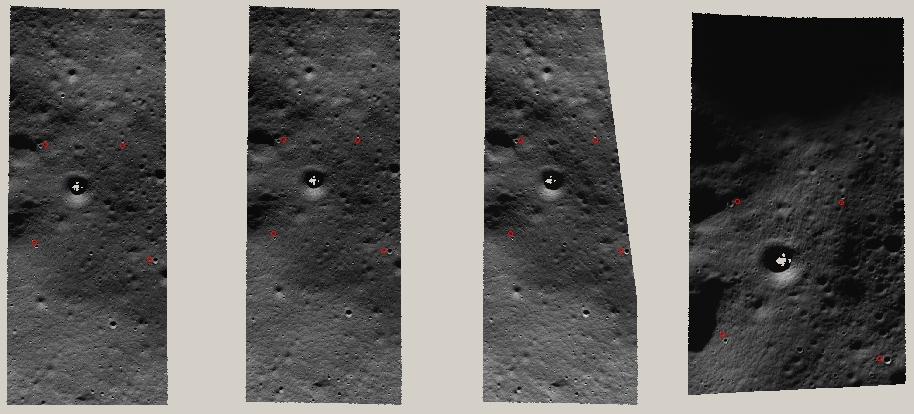
\includegraphics[width=7in]{images/sfs3.jpg}
    \caption[sfs]{An illustration of how interest points are picked manually for the purpose of bundle adjustment and then SfS.}
    \label{fig:sfs3}
  \end{center}
\end{figure}

A good sanity check to ensure that at this stage cameras are aligned
properly is to map-project using the newly obtained camera adjustments
and then overlay the obtained images in the GUI.  The features in all
images should be perfectly on top of each other.
\begin{verbatim}
  for f in A B C D; do 
    mapproject --tr 4 run_stereo_noba_sub4/run-DEM.tif ${f}_crop_sub4.cub  \
     ${f}_crop_sub4_v2.tif --tile-size 128 --bundle-adjust-prefix run_ba_sub4/run
  done
\end{verbatim}
This will also show where the images overlap, and hence on what portion of the DEM we
can run SfS.

Then we run stereo, followed by SfS. 
\begin{verbatim}
  stereo A_crop_sub4.cub B_crop_sub4.cub run_stereo_yesba_sub4/run             \
    --subpixel-mode 3 --bundle-adjust-prefix run_ba_sub4/run
  point2dem --stereographic --proj-lon -5.7113451 --proj-lat -85.000351        \
    run_stereo_yesba_sub4/run-PC.tif --tr 4
  gdal_translate -srcwin 138 347 273 506 run_stereo_yesba_sub4/run-DEM.tif     \
    run_stereo_yesba_sub4/run-crop1-DEM.tif 
  sfs -i run_stereo_yesba_sub4/run-crop1-DEM.tif A_crop_sub4.cub               \
    C_crop_sub4.cub D_crop_sub4.cub -o sfs_sub4_ref1_th_reg0.12_wt0.001/run    \
    --shadow-thresholds '0.00149055 0.00138248 0.000747531'                    \
    --threads 4 --smoothness-weight 0.12 --initial-dem-constraint-weight 0.001 \
    --reflectance-type 1 --float-exposure --float-cameras --max-iterations 20  \
    --use-approx-camera-models --use-rpc-approximation --crop-input-images     \
    --bundle-adjust-prefix run_ba_sub4/run
\end{verbatim}

We fetch the portion of the LOLA dataset around the current DEM from the
site described earlier, and save it as
\verb#RDR_354E355E_85p5S84SPointPerRow_csv_table.csv#. It is necessary
to align our stereo DEM with this dataset to be able to compare
them. We choose to bring the LOLA dataset into the coordinate system
of the DEM, using:
\begin{verbatim}
  pc_align --max-displacement 280 run_stereo_yesba_sub4/run-DEM.tif             \
    RDR_354E355E_85p5S84SPointPerRow_csv_table.csv -o run_stereo_yesba_sub4/run \
    --save-transformed-source-points
\end{verbatim}

Then we compare to the aligned LOLA dataset the input to SfS and its output:
\begin{verbatim}
  geodiff --absolute -o beg --csv-format '1:lon 2:lat 3:radius_km' \
    run_stereo_yesba_sub4/run-crop1-DEM.tif run_stereo_yesba_sub4/run-trans_source.csv
  geodiff --absolute -o end --csv-format '1:lon 2:lat 3:radius_km' \
    sfs_sub4_ref1_th_reg0.12_wt0.001/run-DEM-final.tif             \
    run_stereo_yesba_sub4/run-trans_source.csv
\end{verbatim}

We see that the mean error between the DEM and LOLA goes down, after SfS,
from  1.14~m to 0.90~m, while the standard deviation decreases from
1.18~m to 1.06~m.

\section{Running SfS with an external initial guess DEM and extreme illumination}

Here we will illustrate how SfS can be run in a very difficult
situation. We chose a site very close to the Lunar South Pole, at around
$89.7^\circ$ South. We used an external DEM as an initial guess terrain,
in this case the LOLA gridded DEM, as such a DEM has values in in
permanently shadowed regions. The terrain size is 5 km by 5 km at 1
meter/pixel (we also ran a 10 km by 10 km region in the same location).

Here the topography is very steep, the shadows are very long and vary
drastically from image to image, and some portions of the terrain show
up only in some images. All this makes it very hard to register images
to each other and to the ground. We solved this by choosing very carefully
a large set of representative images. 

The first step is to fetch the underlying LOLA DEM. We use the 20
meter/pixel one, resampled to 1 meter/pixel, creating a DEM
named \texttt{ref.tif}.

\begin{verbatim}
   wget http://imbrium.mit.edu/DATA/LOLA_GDR/POLAR/IMG/LDEM_80S_20M.IMG
   wget http://imbrium.mit.edu/DATA/LOLA_GDR/POLAR/IMG/LDEM_80S_20M.LBL
   pds2isis from = LDEM_80S_20M.LBL to = ldem_80s_20m.cub
   image_calc -c "0.5*var_0" ldem_80s_20m.cub -o ldem_80s_20m_scale.tif
   gdal_translate -projwin -7050.500 -5759.500 -1919.500 -10890.500 \
     ldem_80s_20m_scale.tif ldem_80s_20m_scale_crop.tif
   gdalwarp -r cubicspline -tr 1 1 ldem_80s_20m_scale_crop.tif ref.tif
\end{verbatim}

Note that we scaled its heights by 0.5 per the information in the LBL file.

By far the hardest part of this exercise is choosing the images. We
downloaded several hundred of them by visiting the web site noted
earlier and searching by the longitude-latitude bounds. The .IMG images
were converted to .cub as before, and they were mapprojected onto the
reference DEM, initially at a lower resolution to get a preview of
things. 

The mapprojected images were mosaicked together using
\texttt{dem\_mosaic} with the option \texttt{-\/-block-max}, with a
large value of \texttt{-\/-block-size} (larger than the image size), and
using the \texttt{-\/-t\_projwin} option to specify the region of
interest (in \texttt{stereo\_gui} one can find this region by selecting
it with Control-Mouse).  When the mosaicking tool runs, the sum of
pixels in the current region for each image will be printed to the
screen. Images with a positive sum of pixels are likely to contribute to
the desired region.

The obtained subset of images should be sorted by the Sun azimuth (this
angle is printed when running \texttt{sfs} with the \texttt{-\/-query}
option on the .cub files). Out of those, the following were kept:

\begin{verbatim}
  M114859732RE.cal.echo.cub       73.1771
  M148012947LE.cal.echo.cub       75.9232
  M147992619RE.cal.echo.cub       78.7806
  M152979020RE.cal.echo.cub       96.895
  M117241732LE.cal.echo.cub       97.9219
  M152924707RE.cal.echo.cub       104.529
  M150366876RE.cal.echo.cub       104.626
  M152897611RE.cal.echo.cub       108.337
  M152856903RE.cal.echo.cub       114.057
  M140021445LE.cal.echo.cub       121.838
  M157843789LE.cal.echo.cub       130.831
  M157830228LE.cal.echo.cub       132.74
  M157830228RE.cal.echo.cub       132.74
  M157809893RE.cal.echo.cub       135.604
  M139743255RE.cal.echo.cub       161.014
  M139729686RE.cal.echo.cub       162.926
  M139709342LE.cal.echo.cub       165.791
  M139695762LE.cal.echo.cub       167.704
  M142240314RE.cal.echo.cub       168.682
  M142226765RE.cal.echo.cub       170.588
  M142213197LE.cal.echo.cub       172.497
  M132001536LE.cal.echo.cub       175.515
  M103870068LE.cal.echo.cub       183.501
  M103841430LE.cal.echo.cub       187.544
  M142104686LE.cal.echo.cub       187.765
  M162499044LE.cal.echo.cub       192.747
  M162492261LE.cal.echo.cub       193.704
  M162485477LE.cal.echo.cub       194.662
  M162478694LE.cal.echo.cub       195.62
  M103776992RE.cal.echo.cub       196.643
  M103776992LE.cal.echo.cub       196.643
\end{verbatim}

(the Sun azimuth is shown on the right, in degrees). These were then mapprojected
onto the reference DEM at 1 m/pixel using the South Pole stereographic
projection specified in this DEM. The \texttt{parallel\_bundle\_adjust}
tool is employed to co-register the images and correct camera errors. 

\begin{verbatim}
     parallel_bundle_adjust --processes 8 --ip-per-tile 1000 --overlap-limit 30   \
       --num-iterations 10 --num-passes 2 --min-matches 1                         \
       <images> --mapprojected-data '<mapprojected images> ref.tif' -o ba/run
\end{verbatim}

For bundle adjustment we in fact used even more images that overlap
with this area, but likely this set is sufficient, and it is this set
that was used later for shape-from-shading. 
Here more bundle
adjustment iterations are desirable, but this step takes too long. And a large
\texttt{-\/-ip-per-tile} can make a difference in images with rather
different illumination conditions. 

It is very important to keep a lot of images in bundle adjustment, to ensure
that there are enough overlaps and sufficiently similar illumination conditions
among them for bundle adjustment to succeed. Later, just a subset can be used
for shape-from-shading, enough to cover the entire region, preferable with
multiple illumination conditions at each location. 

A very critical part of the process is aligning the obtained cameras to the ground:

\begin{verbatim}
    pc_align --max-displacement 400 --save-transformed-source-points              \
      --compute-translation-only --csv-format '1:lon 2:lat 3:height_above_datum'  \
      ref.tif ba/run-final_residuals_no_loss_function_pointmap_point_log.csv      \
      -o ba/run 
\end{verbatim}

The value of \texttt{-\/-max-displacement} could be too high perhaps, it
is suggested to also experiment with half of that and keep the result
that has the smaller error.

The flag \texttt{-\/-compute-translation-only} turned out to be
necessary as \texttt{pc\_align} was introducing a bogus rotation. 

The obtained alignment transform can be applied to the cameras to make them aligned
to the ground:

\begin{verbatim}
    mkdir -p ba_align
    /bin/cp -fv ba/run* ba_align
    bundle_adjust --skip-matching --num-iterations 0 --force-reuse-match-files \
      --num-passes 1 --initial-transform ba/run-transform.txt                  \
      --input-adjustments-prefix ba/run <images> -o ba_align/run
\end{verbatim}

The images should now be projected onto this DEM as:

\begin{verbatim}
   mapproject --tr 1 --bundle-adjust-prefix ba_align/run \
     ref.tif image.cub image.map.tif
\end{verbatim}

It is very important to overlay the obtained images and ensure that they
are precisely on top of each other and on top of the LOLA DEM. 

There are occasions in which the alignment transform is still not accurate
enough. Then, one can refine the cameras using the reference terrain as
a constraint in bundle adjustment:

\begin{verbatim}
    mkdir -p ba_align_ref
    /bin/cp -fv ba_alin/run* ba_align_ref
    bundle_adjust --skip-matching --num-iterations 5 --force-reuse-match-files   \
      --num-passes 1 --input-adjustments-prefix ba_align/run <images>            \
      --camera-weight 0 --heights-from-dem ref.tif --heights-from-dem-weight 0.1 \ 
      -o ba_align_ref/run
\end{verbatim}

After mapprojecting with the newly refined cameras in \texttt{ba\_align\_ref}
any residual alignment errors should go away. The value used for
\textt{-\/-heights-from-dem-weight} may need some experimentation. The reference
DEM has vertical error as well, so of this value is too high, it may bind too
tightly to this somewhat innacurate DEM. Yet, making it too low may not
constrain sufficiently the uncertainty that exists in the height of triangulated
points after bundle adjustment, which is rather high since LRO NAC is mostly looking
down so the convergence angle among any rays going through matching interest points
is small.

It is suggested that the user examine the file
\begin{verbatim}
  ba_align_ref/run-final_residuals_no_loss_function_pointmap_point_log.csv
\end{verbatim}

to see if the reprojection errors (column 4) are reasonably small, say mostly
on the order of 0.1 pixels. The triangulated point cloud
from this file should also hopefully be close to the reference DEM. Their
difference is found as:
\begin{verbatim}
  geodiff --absolute                                                         \
    --csv-format '1:lon 2:lat 3:height_above_datum' ref.tif                  \
    ba_align_ref/run-final_residuals_no_loss_function_pointmap_point_log.csv \
    -o ba_align_ref/run
\end{verbatim}

Some of the differences that will be saved to disk are likely outliers,
but mostly they should be small, perhaps on the order of 1 meter.

If, even after this step, the mapprojected images fail to be perfectly
on top of each other, or areas with poor coverage exist, more images
with intermediate illumination conditions and more terrain coverage
should be added and the process should be restarted. As a last resort,
any images that do not overlay correctly must be removed from
consideration for the shape-from-shading step.

Next, SfS follows:

\begin{verbatim}
   parallel_sfs -i ref.tif <images> --shadow-thresholds '<thresholds>'  \
     --bundle-adjust-prefix ba_align_ref/run -o sfs/run                 \ 
     --use-approx-camera-models --crop-input-images                     \
     --blending-dist 10 --min-blend-size 100 --threads 4                \
     --smoothness-weight 0.12 --initial-dem-constraint-weight 0.0001    \
     --reflectance-type 1 --max-iterations 5  --save-sparingly          \
     --tile-size 200 --padding 50 --num-processes 20                    \
     --nodes-list <machine list>
\end{verbatim}

The shadow thresholds were chosen here to be 0.003.

The first step that will happen when this is launched is computing the
exposures. That one can be a bit slow, and can be done offline, using
the flag \texttt{-\/-compute-exposures-only} in this tool, and then the
computed exposures can be passed to the command above via the
\texttt{-\/-image-exposures-prefix} option.

The obtained shape-from-shading terrain should be studied carefully to
see if it shows any systematic shift or rotation compared to the initial
LOLA gridded terrain. If necessary, it can be re-aligned to it using
\texttt{pc\_align} (perhaps using only the compute translation flag).

If SfS is run on multiple overlapping terrains, it is unavoidable that
the output terrains will be offset in respect to each other, hopefully
by no more than several meters or tens of meters. After aligning them to
LOLA as well as possible, they can also be aligned to each other if they
have enough overlap, using the \texttt{pc\_align} option
\texttt{-\/-initial-transform-from-hillshading} (whose value should be
either 'translation' or 'rigid', unless a scale change is suspected).
One should consider using zero iterations here or disabling the
rotations in case it appears that this tool is overeager and the aligned
DEM moves in unacceptable ways.

Lastly, the \texttt{geodiff} tool can be deployed to see how the SfS DEM
compares to the initial guess or to the raw ungridded LOLA measurements.

\section{Insights for getting the most of SfS}
\label{sfs:insights}

Here are a few suggestions we have found helpful when running \texttt{sfs}:

\begin{itemize}{}

\item First determine the appropriate smoothing weight $\mu$ by running a
  small clip, and using just one image. A value between 0.06 and 0.12 seems to work 
  all the time with LRO NAC, even when the images are subsampled. The other weight, $\lambda,$ can
  be set to something small, like $0.0001.$ This can be increased to $0.001$ if noticing
  that the output DEM strays too far. 

\item As stated before, more images with more diverse illumination conditions
  result in more accurate terrain. Ideally there should be at least 3 images, with the shadows
  being, respectively, on the left, right, and then perhaps missing or small. 

\item Bundle-adjustment for multiple images is crucial, to eliminate
  camera errors which will result in \texttt{sfs} converging to a local
  minimum. This is described in section \ref{sfs-lola}.

\item Floating the albedo (option \texttt{-\/-float-albedo}) can
  introduce instability and divergence, it should be avoided unless
  obvious albedo variation is seen in the images.

\item Floating the DEM at the boundary (option
  \texttt{-\/-float-dem-at-boundary}) is also suggested to be avoided.

\item Overall, the best strategy is to first use SfS for a single image
  and not float any variables except the DEM being optimized, and then
  gradually add images and float more variables and select whichever
  approach seems to give better results.

\item If an input DEM is large, it may not be completely covered by a
  single set of imagery with various illumination conditions.  It should
  then be broken up into smaller regions (with overlap), the SfS problem
  can be solved on each region, and then every output terrain can be
  transformed using \texttt{pc\_align} into LOLA's global coordinate
  system, where they can be mosaicked together using
  \texttt{dem\_mosaic}. Or, \texttt{sfs} can be run not on one clip, but
  on an entire collection of clips covering this area to get the
  adjustments, and then \texttt{parallel\_sfs} can be run as described in
  the previous section. 

  The easier case is when at least the two images in the stereo pair
  cover the entire terrain. Then, portions of this terrain can be used
  as an initial guess for each SfS sub-problem (even as the other images
  used for SfS change), the results can be mosaicked, and the alignment
  to LOLA can happen just once, after mosaicking. This approach is
  preferable, if feasible, as alignment to LOLA is more accurate if the
  terrain to align is larger in extent.

\item The \texttt{mapproject} program can be used to map-project each image
  onto the resulting SfS DEM (with the camera adjustments solved using
  SfS). These orthoimages can be mosaicked using \texttt{dem\_mosaic}. If the
  \texttt{-\/-max} option is used with this tool, it create a mosaic with
  the most illuminated pixels from this image. If during SfS the camera
  adjustments were solved accurately, this mosaic should have little or no
  blur.

\item For challenging datasets it is suggested to first work at 1/4th of
the full resolution (the resolution of an ISIS cube can be changed using
the \texttt{reduce} command, and the DEM can be made coarser with
\texttt{gdalwarp} or by converting it to a cloud with \texttt{pc\_align}
with zero iterations and then regenerated with \texttt{point2dem}).
This should make the whole process perhaps an order of magnitude
faster. Any obtained camera adjustment files are still usable at the
full resolution (after an appropriate rename), but it is suggested that
these adjustments be reoptimized using the full resolution cameras,
hence these should be initial guesses for \texttt{bundle\_adjust}'s 
\texttt{-\/-input-adjustments-prefix} option.

\end{itemize}
